\documentclass[11pt]{article}
\usepackage[margin=2.5cm]{geometry}
\usepackage{graphicx}
\usepackage{booktabs}
\usepackage{amsmath}
\usepackage{caption}
\usepackage[colorlinks=true,linkcolor=blue,citecolor=blue]{hyperref}

\title{The Final Chosen Controller: \texttt{plain\_seed123}\\
\large Methodology, Simulation Results, and Hardware Deployment Summary}
\author{}
\date{\today}

\begin{document}
\maketitle

\noindent This document is a self-contained methodology and results write-up for the single
genome family carried forward to hardware deployment out of the full "beat the LJ baseline"
investigation: \textbf{\texttt{plain\_seed123}}, in its \emph{unclamped} form (best simulation
performance) and its \emph{clamped} form (retrained from scratch with a hard inter-agent
safety reflex, for physical deployment). It is kept deliberately isolated from
\texttt{summary.tex} (which documents the broader search across ablations and other
candidate genomes) and is intended to be dropped into Overleaf as-is or cannibalized for a
Methodology/Results section. All figures live in \texttt{figures/} alongside this file, each
exported as \texttt{.pdf}/\texttt{.svg}/\texttt{.png}. For the complete search history that
led to this choice -- including the other three candidate genomes considered and why they
were \emph{not} chosen -- see
\texttt{hardware\_transfer\_test/BEAT\_BASELINE\_INVESTIGATION\_LOG.md}.

\section*{Figure import guide}
\begin{center}
\begin{tabular}{@{}lll@{}}
\toprule
\textbf{File (basename, no extension)} & \textbf{Content} & \textbf{Used in} \\
\midrule
\texttt{safety\_clamp\_scale\_function} & clamp scale function $C(g)$ & \S\ref{sec:clamp} \\
\texttt{paper\_fig5a\_distance\_vs\_battery\_n20\_plain\_seed123} & Fig.~5a analog, $n{=}20$ & \S\ref{sec:fig5a} \\
\texttt{paper\_fig6\_trajectory\_comparison\_plain\_seed123} & Fig.~6 analog, $n{=}2$ vs.\ $20$ & \S\ref{sec:fig6} \\
\texttt{n\_agents\_sweep\_distance\_battery\_plain\_seed123} & distance/battery vs.\ swarm size & \S\ref{sec:nsweep} \\
\texttt{n\_agents\_sweep\_position\_change\_plain\_seed123} & front-rank exchange rate vs.\ swarm size & \S\ref{sec:nsweep} \\
\texttt{n\_agents\_sweep\_battery\_equity\_plain\_seed123} & battery-sharing equity vs.\ swarm size & \S\ref{sec:nsweep} \\
\texttt{metric1\_reciprocity\_scatter}, \texttt{metric1\_seed\_sweep\_n20} & Voelkl reciprocity & \S\ref{sec:leadership} \\
\texttt{metric2\_hierarchy\_summary}, \texttt{metric2\_seed\_sweep\_n20} & Nagy hierarchy network & \S\ref{sec:leadership} \\
\texttt{metric3\_front\_occupancy}, \texttt{metric3\_exchange\_rate}, \texttt{metric3\_seed\_sweep\_n20} & front-rank occupancy/exchange & \S\ref{sec:leadership} \\
\texttt{metric4\_exchange\_rate\_filtered}, \texttt{metric4\_seed\_sweep\_n20} & persistence-filtered hand-offs & \S\ref{sec:leadership} \\
\bottomrule
\end{tabular}
\end{center}
(Most leadership-metric figures live in \texttt{leadership\_analysis\_plain\_seed123/} --
kept isolated from the original three-condition pipeline's \texttt{leadership\_analysis/} per
the same isolation request -- except the two embedded directly in this document
(\texttt{metric3\_exchange\_rate\_plain\_seed123}, \texttt{metric4\_exchange\_rate\_filtered\_plain\_seed123}),
copied into \texttt{figures/} for a self-contained Overleaf upload.)

\section{Methodology}

\subsection{Controller and evolutionary training (shared by both variants)}
Both variants share the identical architecture, sensor model, and CMA-ES configuration
documented in full in \texttt{summary.tex} \S2.1: a 10-input, two-hidden-layer (10 units
each), 2-output Hebbian-plasticity MLP, weights updated online every step by
$\Delta w_{ij} = \mu(A_{ij}n_in_j + B_{ij}n_i + C_{ij}n_j + D_{ij})$, $\mu=0.1$, with the
$(A,B,C,D)$ coefficients (880 real values, bounded $[-5,5]$) evolved by CMA-ES (population 30,
fitness = median efficiency over 3 seed repeats, $n_{\text{agents}}=20$ candidate evaluation
swarm, wind grid $50\times50$).

\subsection{The 2-stage \texttt{walk\_upwind} curriculum}
\label{sec:curriculum}
Both variants use a 2-stage curriculum -- \texttt{walk\_upwind} (100 generations, wind
enabled, reward $=w_d\cdot(\overline{x},\overline{y})\cdot(-1,0)$, $w_d=16$) directly into
\texttt{save\_battery\_avoid\_all} (200 generations, full battery + wall + inter-robot
collision terms from the start, $w_b=5.0$, $w_c=250.0$) -- skipping the separate
wall-only-collision intermediate stage that the original paper-replication genomes used. This
was found, after a systematic search across roughly thirty other training/evaluation
configurations (drain-holiday variants, zero-collision-signal training, increased wind-drag
coupling, etc. -- see the investigation log), to be the first curriculum structure capable of
producing genomes that reliably beat the rule-based LJ baseline on both distance and battery
simultaneously, not just on average. Seed 123 was one of two seeds (of five independently
trained) that reached this reliable tier under the plain-drain collision-cost regime used
here.

\subsection{Unclamped training}
\texttt{plain\_seed123} (unclamped) was trained with no additional safety mechanisms
(\texttt{HEBBIAN\_SAFETY\_CLAMP\_ENABLED=False}), standard (non-refunded) battery drain
throughout, $n_{\text{agents}}=20$, seed 123. Genome:
\texttt{hardware\_transfer\_test/final/plain\_seed123/genome\_trained\_n20.npy}.

\subsection{Clamped training: why retrain from scratch}
\label{sec:clamp}
Real robots have no physical compliance, so a genome with no trained-in collision-avoidance
reflex is a real hardware risk. Two approaches were considered:

\paragraph{Bolt-on deployment-only governor -- tested and rejected.} A speed governor applied
\emph{after} the (already-trained, unclamped) genome's own $v,w$ output was tested at six
band widths, from the training-grade $g_{\text{out}}{=}0.30\text{m}$/$g_{\text{in}}{=}0.05\text{m}$
down to a razor-thin $0.005\text{m}/0.001\text{m}$ near-contact-only band. \textbf{Every band
width collapsed distance to roughly 10--16\% of unclamped} (e.g.\ 18.57m~$\to$~1.8--3.1m for
this genome) via a gridlock failure mode: any discrepancy between the network's commanded
speed and what actually executes appears to derail its online Hebbian update into a
degenerate fixed point, regardless of how rarely the discrepancy occurs. No band width is
viable as a pure bolt-on.

\paragraph{Retrained from scratch instead.} \texttt{plain\_seed123\_clamped} repeats
\S\ref{sec:curriculum}'s exact curriculum with the hard forward-speed clamp active
\emph{during} evolution, so CMA-ES can learn to route around it -- the same approach already
validated by the original paper-replication \texttt{safety\_clamp\_best} genome. The clamp
(Eq.~\ref{eq:clamp}, Fig.~\ref{fig:clamp}) rescales only the network's commanded forward speed
$v_i$, using the true (uninflated) robot radius $r=0.055$m, leaving turning $\omega_i$
untouched so a braked agent can still steer clear:
\begin{equation}
C(g;\,g_{\text{in}},g_{\text{out}}) = \operatorname{clip}\!\left(\frac{g-g_{\text{in}}}{g_{\text{out}}-g_{\text{in}}},0,1\right),
\qquad v_i^{\text{clamped}} = v_i^{\text{cmd}}\cdot\min\big(C(g_i^{\text{agent}};0.05,0.30),\,C(g_i^{\text{wall}};0.02,0.15)\big)
\label{eq:clamp}
\end{equation}
with $g_i^{\text{agent}}=\min_{j\neq i}(\lVert p_i-p_j\rVert-2r)$ the gap to the nearest other
agent's surface. Training also inflates the collision-\emph{bookkeeping} threshold by
$1.3\times$ (\texttt{HEBBIAN\_MIN\_DIST\_INFLATION}) and applies a soft post-integration
de-overlap push (\texttt{HEBBIAN\_RESOLVE\_COLLISIONS}, strength 0.5, 2 passes) when agents
still end a step overlapping -- see \texttt{summary.tex} \S2.4.1 for the full derivation of
these three mechanisms; \S\ref{sec:clamp-deploy} below covers which of them is portable to
real hardware.

\begin{figure}[h]
\centering
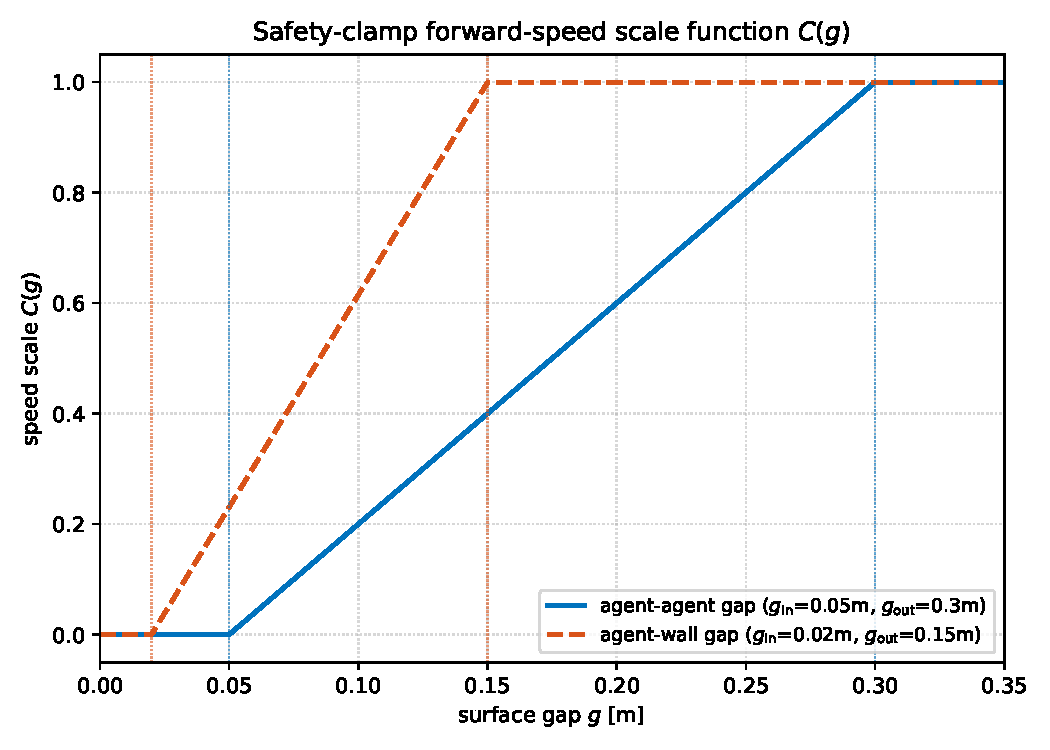
\includegraphics[width=0.65\textwidth]{figures/safety_clamp_scale_function}
\caption{The scale function $C(g)$ for both gap types.}
\label{fig:clamp}
\end{figure}

\paragraph{Cost of the clamp.} Stage-1 (\texttt{walk\_upwind}, distance-only fitness) final
efficiency dropped from 211 (unclamped) to 203 (clamped) for this seed -- a comparatively
small cost. (For contrast, the other two candidate genomes considered lost roughly 60\% of
their stage-1 efficiency under the same clamp -- \texttt{plain\_seed123} happened to be far
less dependent on the tight/fast clustering strategy the clamp forecloses, which is part of
why it survived retraining better than the alternatives; see the investigation log.) Genome:
\texttt{hardware\_transfer\_test/final/plain\_seed123\_clamped/genome\_trained\_n20.npy}.

\subsection{Evaluation protocol}
Identical for both variants unless noted: seed 42 (\texttt{config.HEBBIAN\_DEFAULT\_SEED}) for
single-run/headline figures, seeds 1000--1029 (30 seeds) for statistical figures, wind grid
$50\times50$, default $3.0$m spawn square, standard (non-refunded) battery drain at evaluation
time regardless of training-time drain regime. \texttt{plain\_seed123\_clamped} is evaluated
\emph{with} its clamp/inflation/resolve-collisions settings active (matching how it was
trained); \texttt{plain\_seed123} (unclamped) with all three off.

\section{Simulation Results}

\subsection{Fig.~5a analog: distance vs.\ battery}
\label{sec:fig5a}
\begin{figure}[h]
\centering
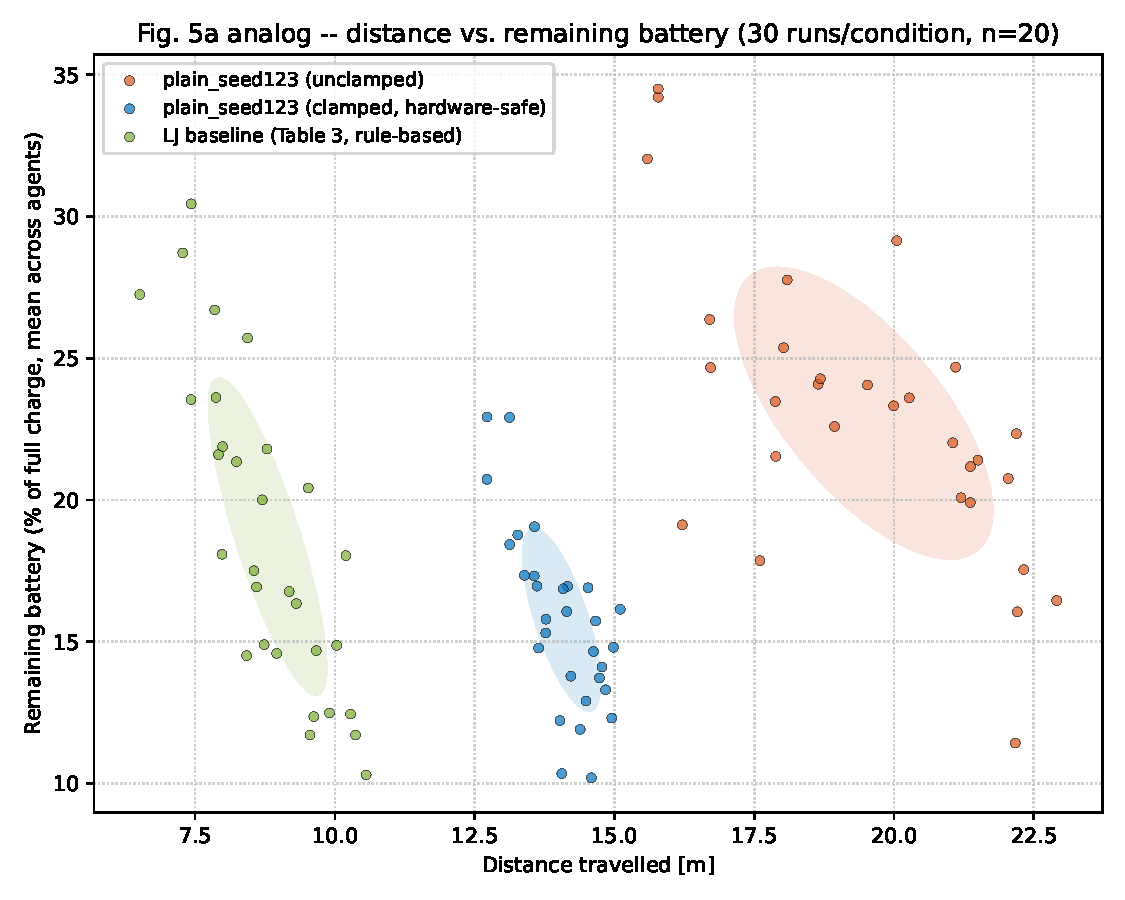
\includegraphics[width=0.85\textwidth]{figures/paper_fig5a_distance_vs_battery_n20_plain_seed123}
\caption{Distance vs.\ remaining battery, 30 seeded runs per condition, $n_{\text{agents}}=20$,
with 1-std confidence ellipses.}
\label{fig:fig5a}
\end{figure}

\begin{table}[h]
\centering
\caption{$n{=}20$, 30 seeds (1000--1029), standard drain physics. Both-beat = fraction of the
30 seeds where that genome's distance \emph{and} battery both exceed the LJ baseline's own
mean (dist~8.81m, batt~18.68\%) simultaneously.}
\label{tab:headline}
\begin{tabular}{@{}lccc@{}}
\toprule
Condition & Distance [m] & Battery [\%] & Both-beat rate \\
\midrule
LJ baseline & $8.80 \pm 1.02$ & $18.71 \pm 5.46$ & -- \\
\texttt{plain\_seed123} (unclamped) & $19.46 \pm 2.25$ & $23.06 \pm 5.02$ & \textbf{25/30 (83\%)} \\
\texttt{plain\_seed123} (clamped) & $14.06 \pm 0.66$ & $15.77 \pm 3.12$ & 5/30 (17\%) \\
\bottomrule
\end{tabular}
\end{table}

\noindent The clamp costs real reliability at evaluation time too (83\%~$\to$~17\%) -- but the
clamped genome still clears the baseline's distance by a comfortable margin (14.06m vs.\
8.81m) and only trails on the battery axis (15.77\% vs.\ 18.71\%), which is why its both-beat
rate is more fragile than the raw distance figure alone would suggest.

\subsection{Fig.~6 analog: trajectories}
\label{sec:fig6}
\begin{figure}[h]
\centering
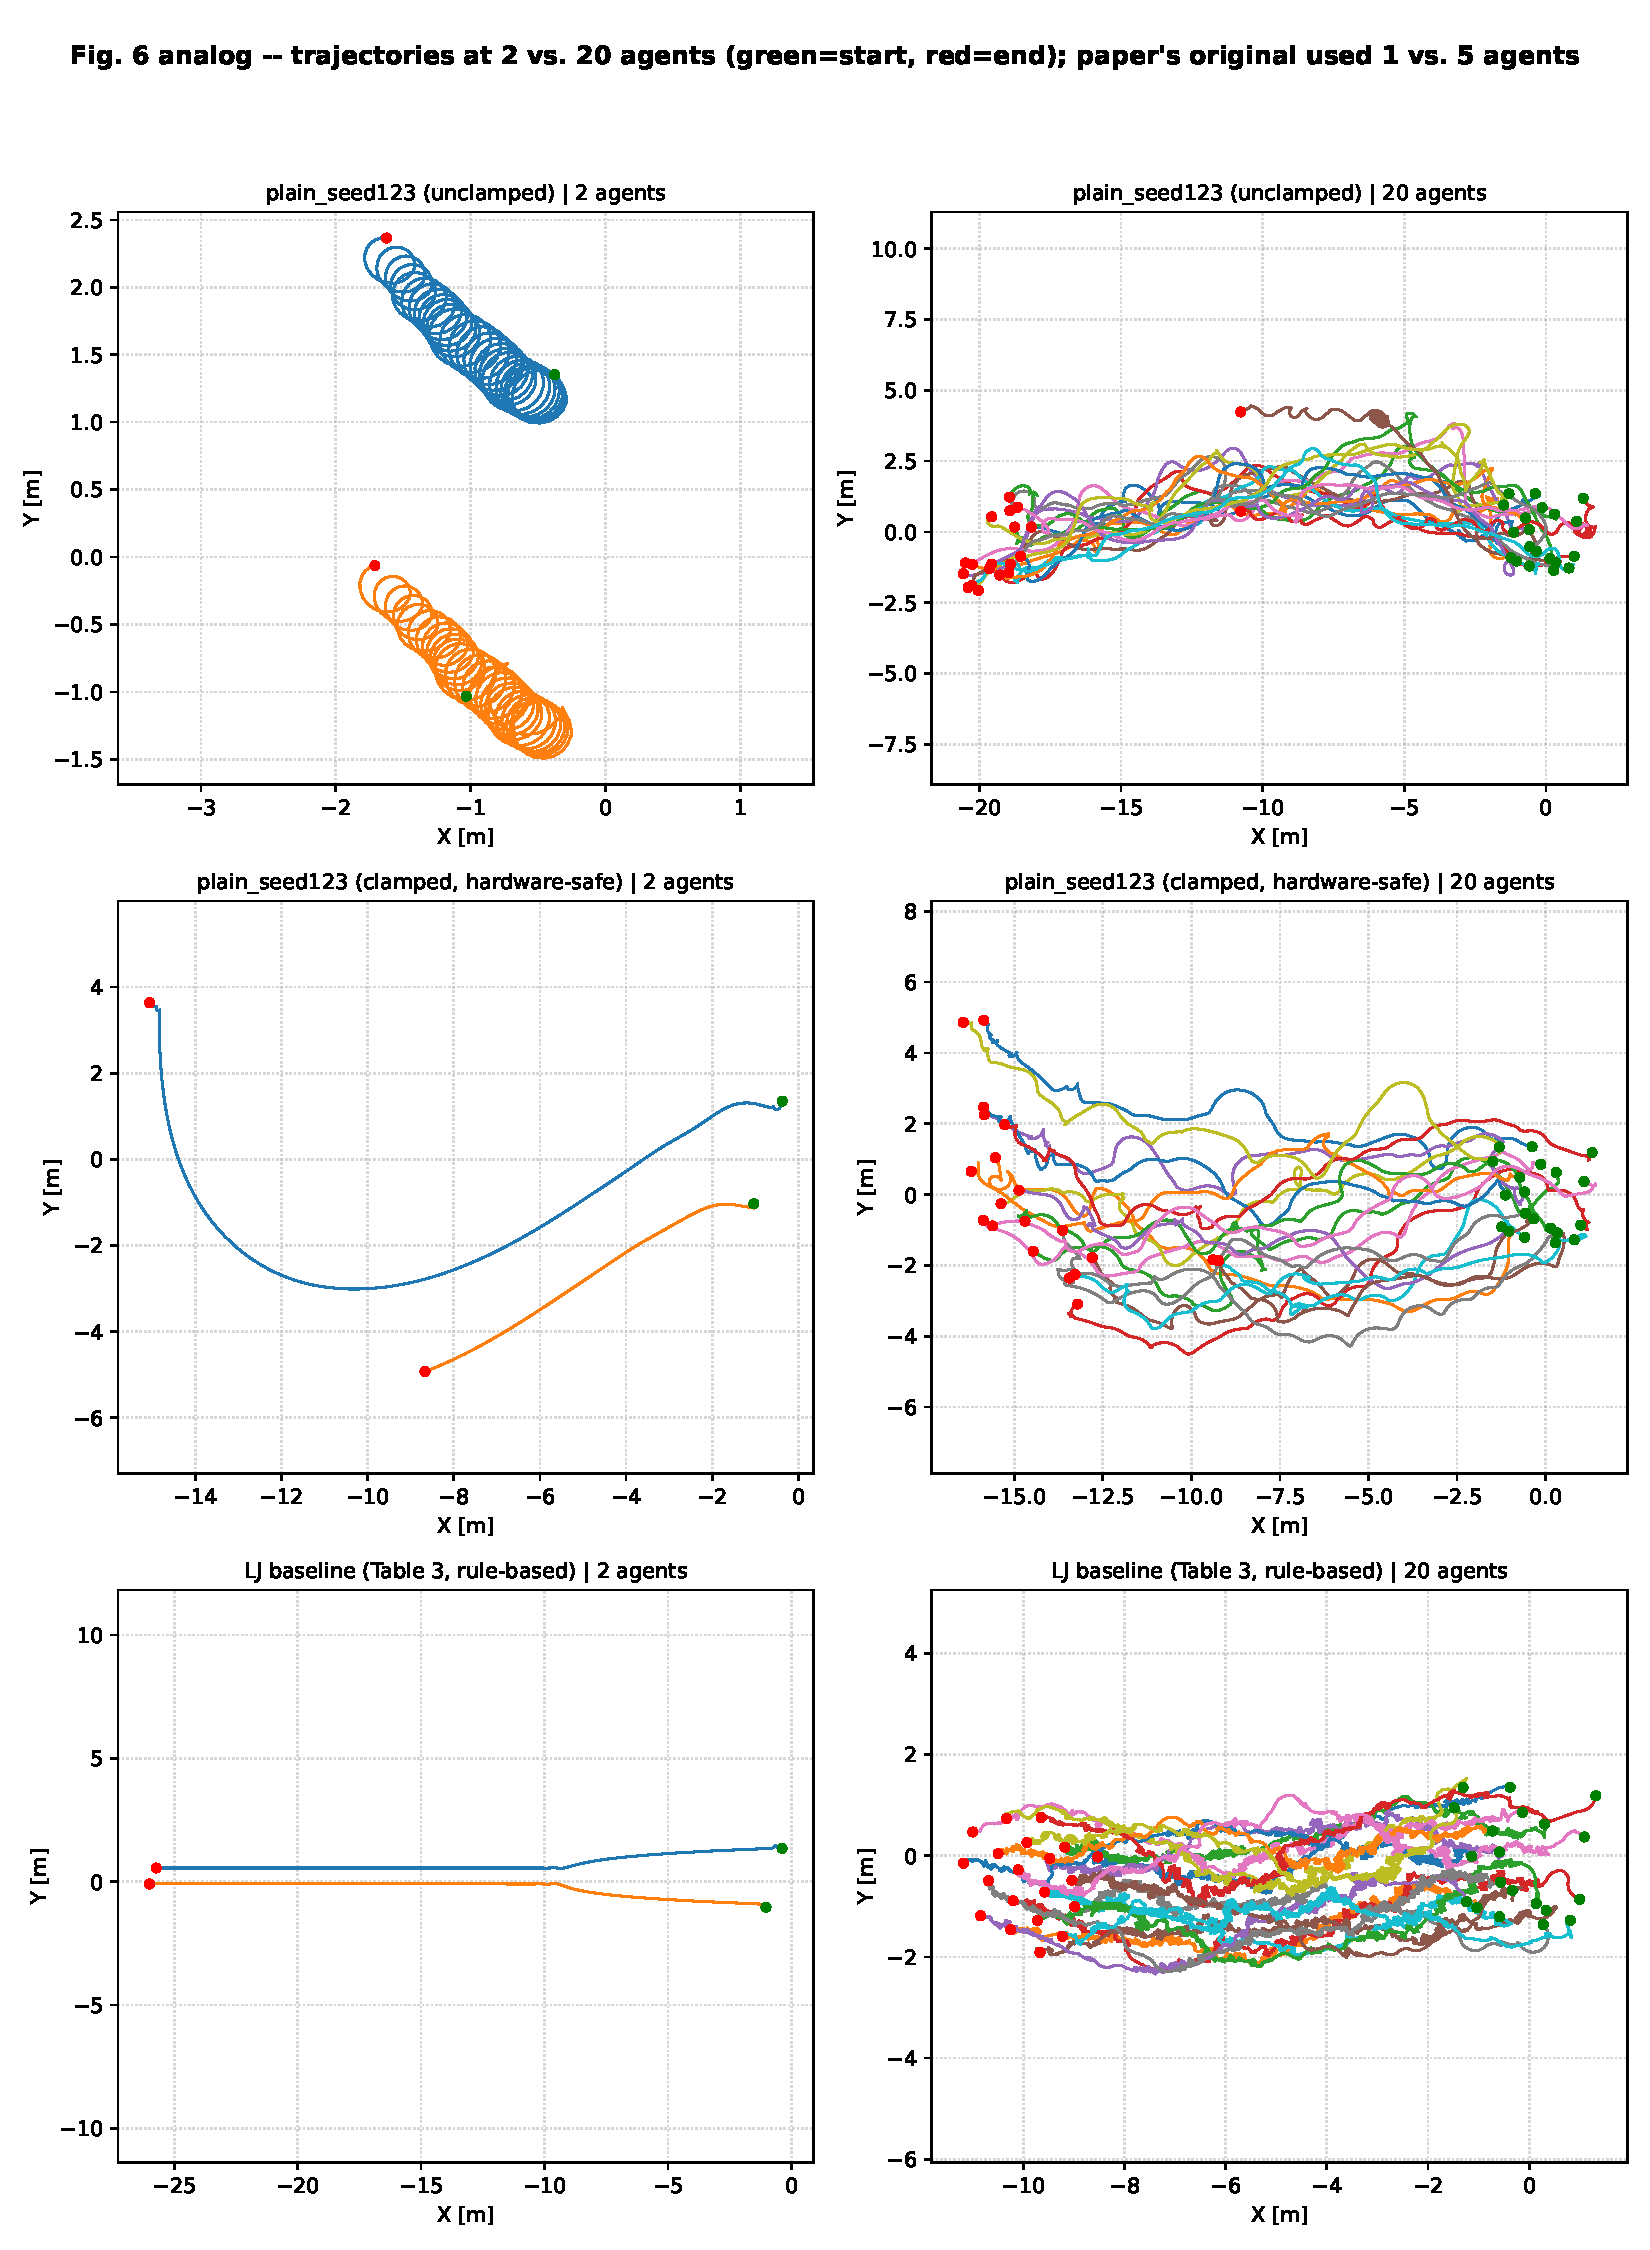
\includegraphics[width=\textwidth]{figures/paper_fig6_trajectory_comparison_plain_seed123}
\caption{Trajectories at $n{=}2$ and $n{=}20$ (green~=~start, red~=~end), seed 42.}
\label{fig:fig6}
\end{figure}

\subsection{Comparison across swarm sizes}
\label{sec:nsweep}
\textbf{The reliable win is specific to $n_{\text{agents}}=20$.} A 30-seed sweep down to
$n_{\text{agents}}\in\{1,2,3,4,5,7,10\}$ found \emph{zero} seeds, for either variant, where
distance and battery both exceeded the LJ baseline at that same swarm size -- only at $n{=}20$
does either genome win reliably (Table~\ref{tab:headline}). This directly bounds what any
hardware trial with fewer robots can be expected to demonstrate (\S\ref{sec:hardware}).

\begin{figure}[h]
\centering
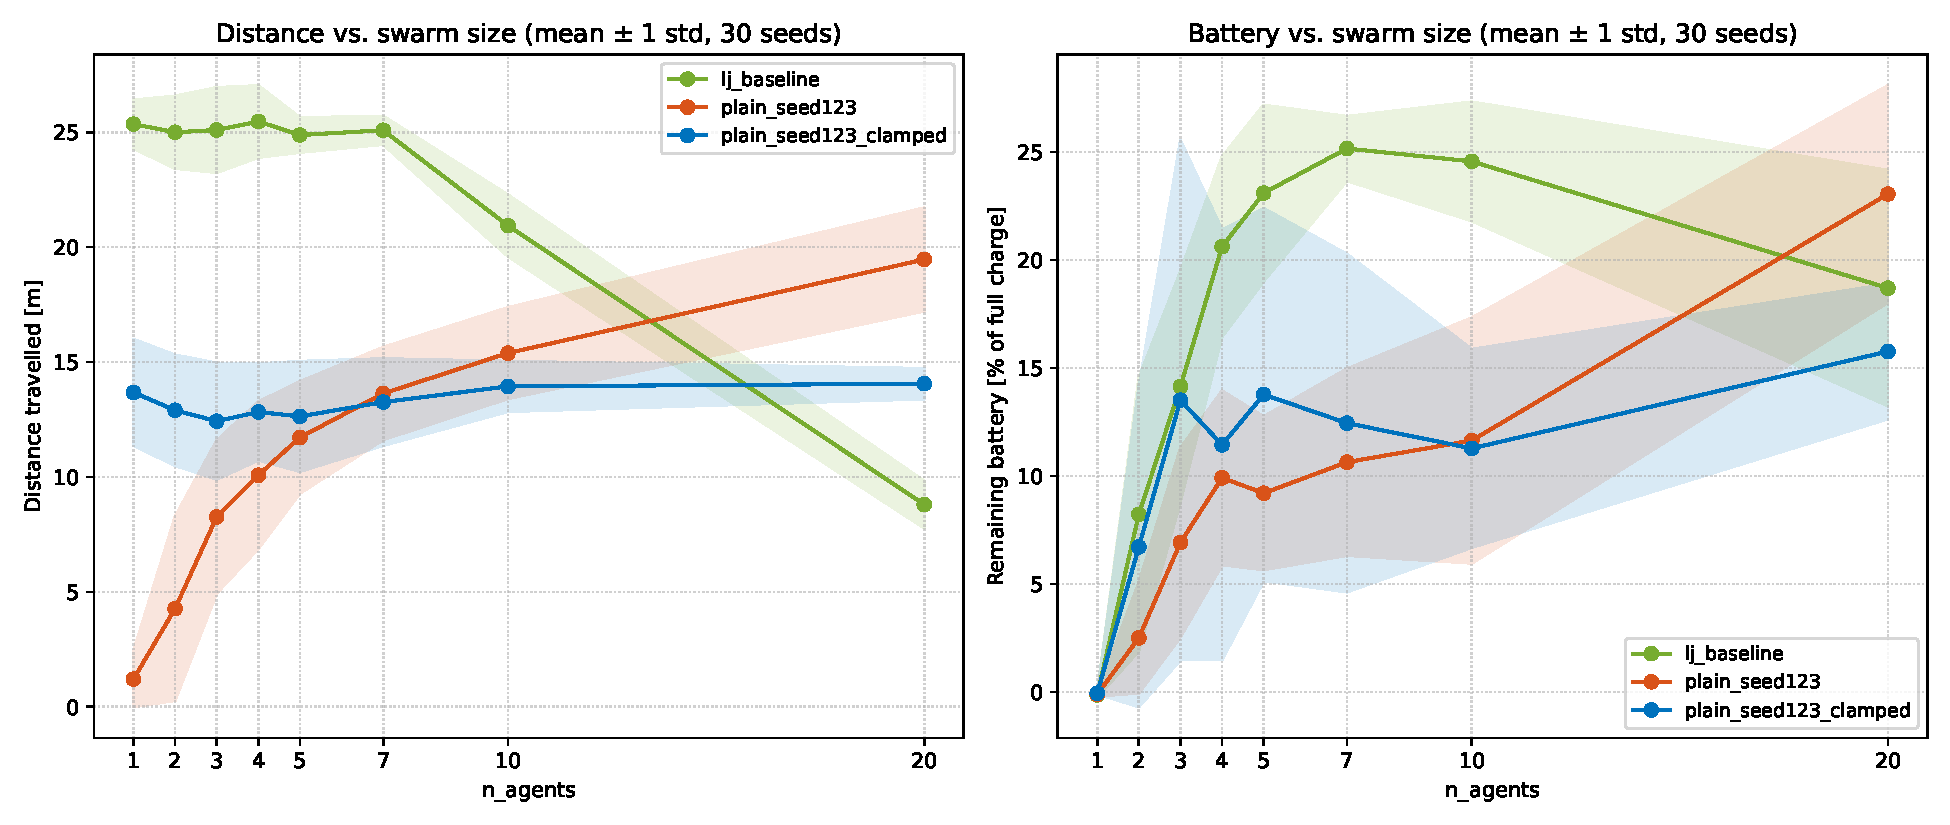
\includegraphics[width=\textwidth]{figures/n_agents_sweep_distance_battery_plain_seed123}
\caption{Distance and battery vs.\ swarm size, mean $\pm$ 1 std over 30 seeds. The LJ
baseline's distance is roughly flat through $n{=}7$ and only collapses toward $n{=}10$--$20$;
both genome variants climb steadily and only cross over near the top of the range.}
\end{figure}

\begin{figure}[h]
\centering
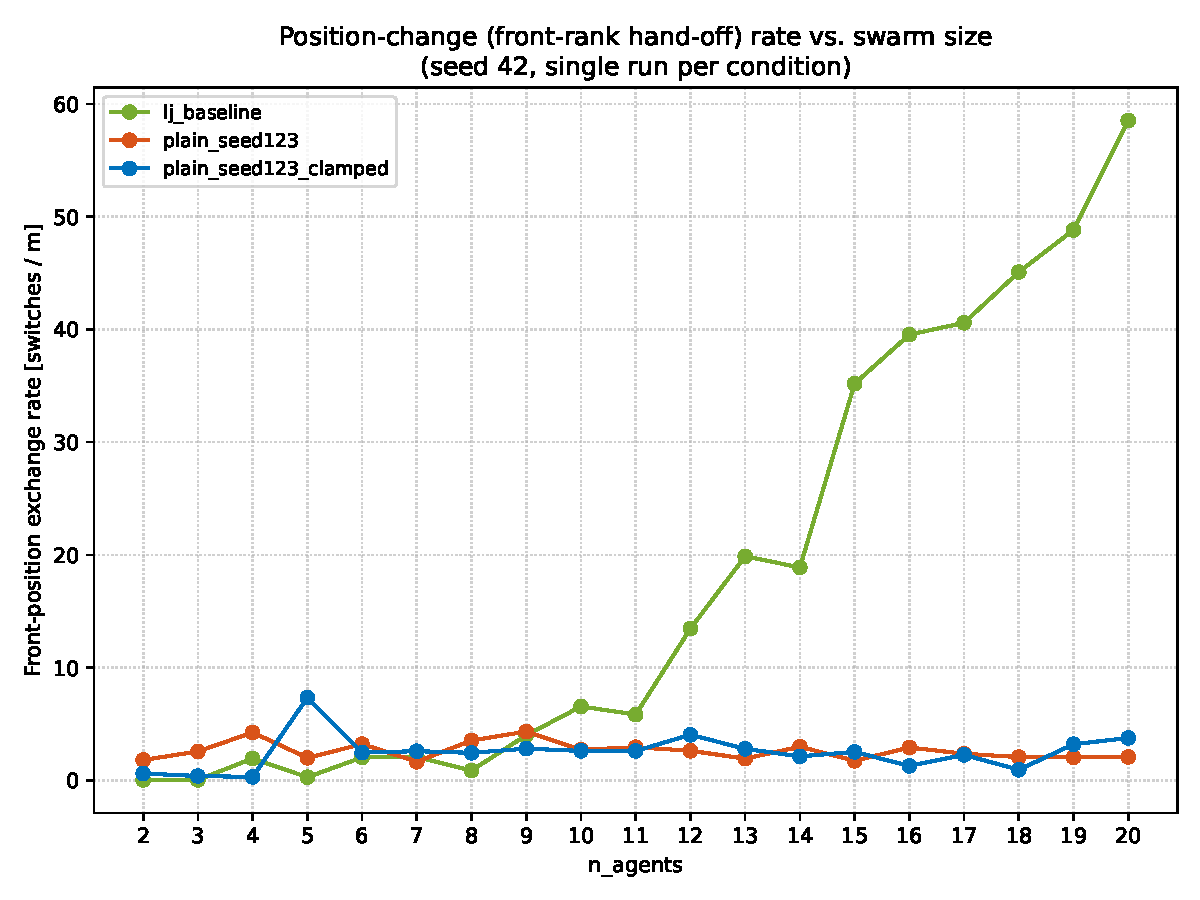
\includegraphics[width=0.8\textwidth]{figures/n_agents_sweep_position_change_plain_seed123}
\caption{Front-rank exchange rate (raw, unfiltered -- see \S\ref{sec:leadership} for why this
needs the persistence-filtered version alongside it) vs.\ swarm size, seed 42.}
\end{figure}

\begin{figure}[h]
\centering
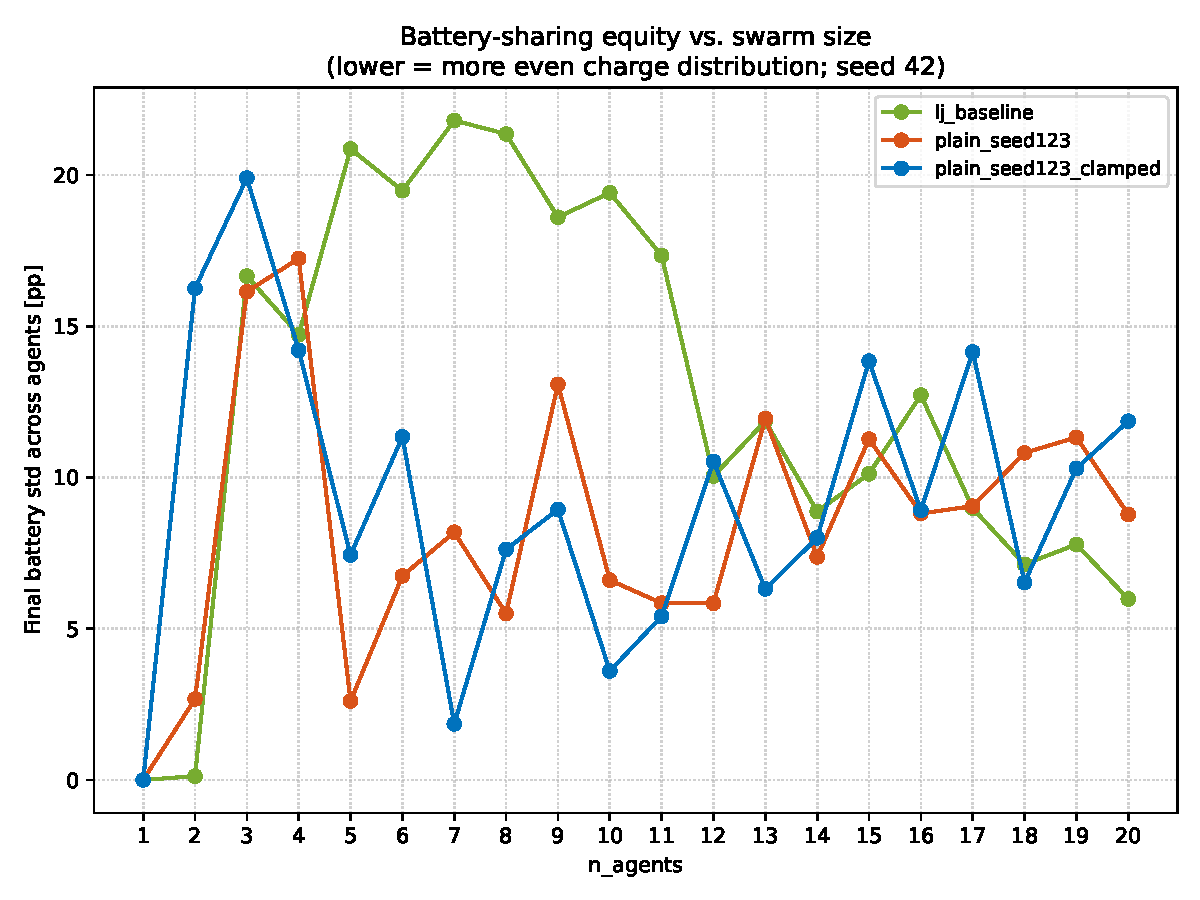
\includegraphics[width=0.8\textwidth]{figures/n_agents_sweep_battery_equity_plain_seed123}
\caption{Final per-agent battery standard deviation vs.\ swarm size (lower = more even charge
distribution across the swarm), seed 42.}
\end{figure}

\subsection{Wall behavior: the deciding factor}
\label{sec:wall}
Not visible in any metric above -- found by reviewing generated videos, then confirmed against
an already-computed but previously-unsurfaced field (\texttt{wall\_collision\_time} in every
archived \texttt{metrics.json}). Expressed as \% of total agent-time budget
($n_{\text{agents}}\times$episode duration) spent within contact margin of a wall:

\begin{table}[h]
\centering
\caption{Wall-contact time as \% of agent-time budget, seed 42, standard physics.}
\begin{tabular}{@{}lcccccccc@{}}
\toprule
$n_{\text{agents}}$ & 1 & 2 & 3 & 4 & 5 & 7 & 10 & 20 \\
\midrule
\texttt{plain\_seed123} (unclamped) & 0.0 & 0.0 & 9.3 & 8.6 & 6.7 & 0.3 & 0.0 & 0.0 \\
\texttt{plain\_seed123} (clamped) & -- & -- & -- & -- & -- & -- & -- & 0.4\footnotemark \\
\bottomrule
\end{tabular}
\end{table}
\footnotetext{$13.0\text{s} / (20\times166.0\text{s}) \approx 0.4\%$, seed 42, $n{=}20$; not
computed at every swarm size for the clamped variant, but consistently negligible where
checked.}

\noindent This is the reason \texttt{plain\_seed123} was chosen over the two other candidate
genomes that emerged from the same search (\texttt{plain\_seed888}, \texttt{drain0\_seed123}),
despite both having a \emph{higher} both-beat rate in simulation (83\% and 97\% respectively,
vs.\ this genome's 83\%): both spend 40--72\% of their agent-time budget parked at a wall at
hardware-relevant swarm sizes, one of them (\texttt{drain0\_seed123}) even when running
completely alone. None of these genomes have any wall-distance sensory input at all -- the
behavior is pure incidental reward-shaping correlation from a fixed-size training arena, not a
real spatial sense, and it varies unpredictably per training seed. See the investigation log
for the full comparison.

\subsection{Leadership / turn-taking metrics}
\label{sec:leadership}
Four metrics from the collective-motion literature, computed identically to
\texttt{summary.tex} \S2.5 (see that section for full definitions and citations
\cite{voelkl2015,nagy2010,mirzaeinia2019,butail2019}), now for
\{\texttt{plain\_seed123}, \texttt{plain\_seed123\_clamped}, \texttt{lj\_baseline}\} across
$n_{\text{agents}}\in\{2,3,4,5,7,10,20\}$ plus a 30-seed robustness sweep at $n{=}10,20$.

\paragraph{Metric 3 vs.\ 4 -- the raw exchange rate is dominated by jitter for the LJ
baseline.} At $n{=}20$, LJ's raw front-identity switch count is 715 of 815 steps (88\%,
Fig.~\ref{fig:m3}) -- but only 8 of those (1.1\%) survive persistence filtering
(\S\ref{sec:leadership}'s Metric 4, $\geq$1.5s dwell). Both genome variants show far fewer raw
switches but a much higher \emph{survival rate} (65\% unclamped, comparable for clamped) --
i.e.\ LJ's huge raw number is mostly rapid jitter among a tightly-bunched front pack, not
genuine sustained leadership change, while the genomes' rarer switches are mostly real. The
clamp does not suppress this real position-changing behavior; if anything it slightly
increases it (raw switches 24~$\to$~55, real switches 10~$\to$~23 at $n{=}20$, seed 42).

\begin{figure}[h]
\centering
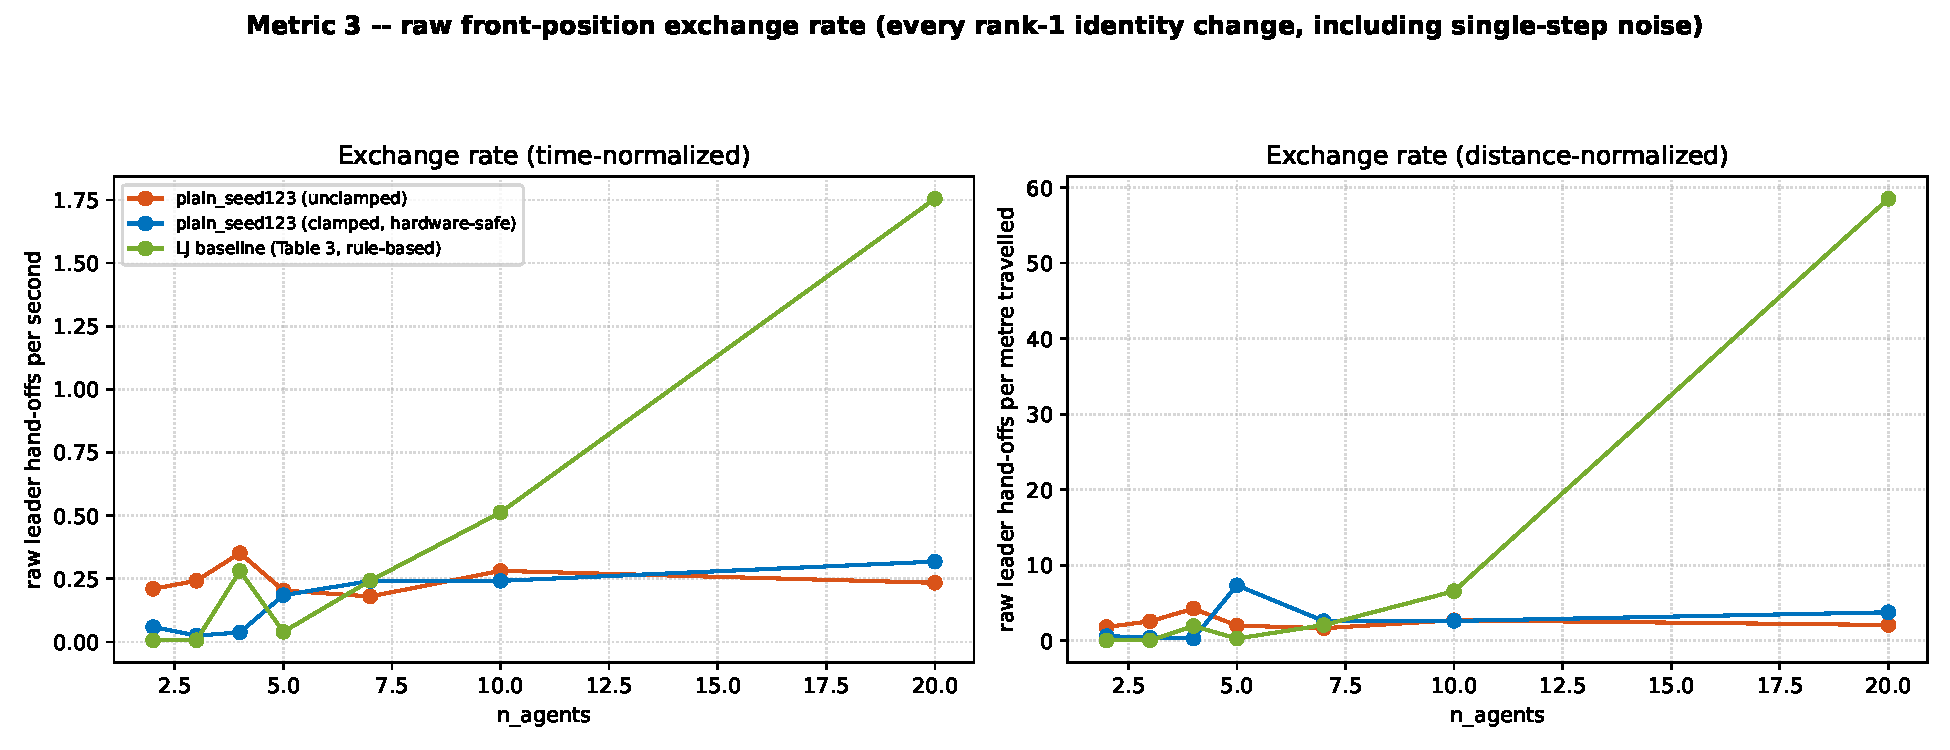
\includegraphics[width=\textwidth]{figures/metric3_exchange_rate_plain_seed123}
\caption{Metric 3 -- raw front-position exchange rate vs.\ swarm size.}
\label{fig:m3}
\end{figure}

\begin{figure}[h]
\centering
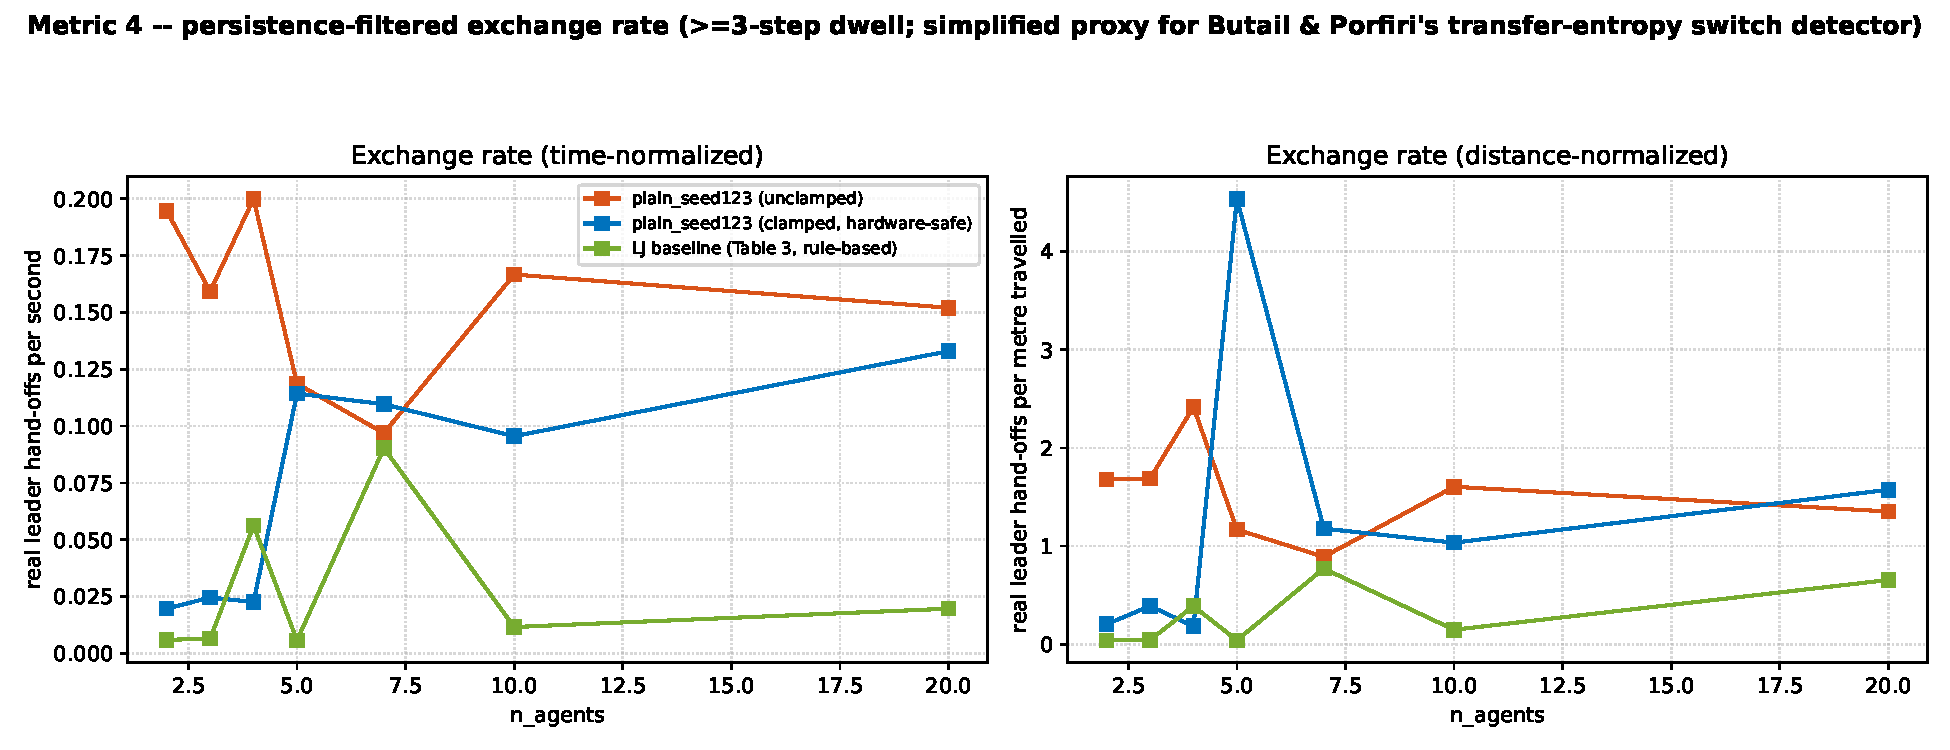
\includegraphics[width=\textwidth]{figures/metric4_exchange_rate_filtered_plain_seed123}
\caption{Metric 4 -- persistence-filtered (real) exchange rate vs.\ swarm size. Both genome
variants sit above the LJ baseline at nearly every swarm size once jitter is filtered out.}
\label{fig:m4}
\end{figure}

\paragraph{Metrics 1/2 -- reciprocity and hierarchy.} Reciprocity ($r$) is negative for all
three conditions at every swarm size tested (Table~\ref{tab:leadership}) -- agents that lead a
lot do not also follow a lot, the opposite of Voelkl et al.'s ibis result, suggesting fairly
fixed leader/follower roles rather than genuine turn-taking by this specific measure, even
though Metric 4 shows real (if infrequent) hand-offs are happening. This is not a
contradiction: reciprocity measures whether roles are \emph{balanced over the whole episode},
while Metric 4 only asks whether the identity of the instantaneous leader changes at all.

\begin{table}[h]
\centering
\caption{Leadership metrics at $n{=}20$, seed 42.}
\label{tab:leadership}
\begin{tabular}{@{}lcccc@{}}
\toprule
Condition & Reciprocity $r$ & Occ.\ entropy & Hier.\ entropy & Hier.\ steepness \\
\midrule
LJ baseline & $-0.109$ & 0.933 & 0.985 & 0.632 \\
\texttt{plain\_seed123} & $-0.389$ & 0.900 & 0.982 & 0.523 \\
\texttt{plain\_seed123\_clamped} & $-0.151$ & 0.379 & 0.989 & 0.594 \\
\bottomrule
\end{tabular}
\end{table}

\noindent 30-seed robustness sweeps at $n{=}10,20$ (\texttt{metric\{1,2,3,4\}\_seed\_sweep\_n\{10,20\}})
confirm these are not one-off seed-42 artifacts -- see
\texttt{leadership\_analysis\_plain\_seed123/} for the full box/strip-plot figures and
per-seed table (\texttt{seed\_sweep\_table\_n\{10,20\}.json}).

\section{Hardware Deployment}
\label{sec:hardware}
\texttt{plain\_seed123\_clamped} is the genome now deployed in
\texttt{ants26\_replication/hardware\_deployment/} (\texttt{plain\_seed123\_clamped\_best.npy}).
Two points specific to this write-up:

\subsection{The clamp must be enforced at deployment time, not just trained-in}
\label{sec:clamp-deploy}
The clamp in \S\ref{sec:clamp} is a \emph{simulation-time} mechanism; training under it shapes
what the network learned, but does not make the network intrinsically collision-avoidant by
itself. Deploying the clamped genome's weights without \emph{also} enforcing the clamp at
runtime would provide no more actual collision safety than the unclamped genome -- confirmed
necessary, not optional, and nearly missed. \texttt{hebbian\_swarm\_experiment.py} now applies
the agent-agent half of Eq.~\ref{eq:clamp} using real OptiTrack-measured neighbor gaps,
combined with the existing wall/corridor governor via $\min(\cdot,\cdot)$ exactly as
Eq.~\ref{eq:clamp} itself combines them. The soft de-overlap mechanism
(\texttt{HEBBIAN\_RESOLVE\_COLLISIONS}) has no real-hardware analog (it teleports/pushes
overlapping agents in software) and is correctly not ported -- only the speed-clamp half is
portable, and it is the half that matters for not colliding at speed.

\subsection{Scope this trial correctly}
Per \S\ref{sec:nsweep}, neither genome variant beats the LJ baseline below $n_{\text{agents}}=20$
in simulation. A real trial with a handful of robots should be scoped as a
\textbf{sim-to-real controller-transfer validation}, not a demonstration of "beats baseline"
-- that claim belongs to the $n{=}20$ simulation results in Table~\ref{tab:headline}, not to
the hardware trial. See \texttt{ants26\_replication/hardware\_deployment/README.md} for the
full deployment configuration, calibration status, and known open risks.

\clearpage
\begin{thebibliography}{9}

\bibitem{mahdavi2026}
Mahdavi et al.\ (2026). \emph{Energy-Efficient Flocking in Self-Organized Robot Swarms}. ANTS
2026 (PoliMi).

\bibitem{voelkl2015}
Voelkl, B., Portugal, S. J., Unsöld, M., Usherwood, J. R., Wilson, A. M., Fritz, J.\ (2015).
Matching times of leading and following suggest cooperation through direct reciprocity during
V-formation flight in ibis. \emph{PNAS}, 112(7), 2115--2120.

\bibitem{nagy2010}
Nagy, M., Ákos, Z., Biro, D., Vicsek, T.\ (2010). Hierarchical group dynamics in pigeon flocks.
\emph{Nature}, 464, 890--893.

\bibitem{mirzaeinia2019}
Mirzaeinia, A., et al.\ (2019). Greedy leading/trailing replacement heuristic for
energy-efficient UAV swarm flight.

\bibitem{butail2019}
Butail, S., Porfiri, M.\ (2019). Detecting switching leadership in collective motion.
\emph{Chaos}, 29(1), 011102.

\end{thebibliography}

\end{document}
